\section{汇编语言简介}

\begin{frame}\ft{机器语言}
机器语言是机器指令的集合。机器指令是计算机可以正确执行的命令,它是一组二进制数字。计算机将其转变为一组高低电平,以使电子器件收到驱动,进行运算。
\end{frame}

\begin{frame}[fragile]\ft{机器语言}
8086CPU完成运算 \lstinline| s=768+12288-1280 |的机器码如下:
\begin{lstlisting}[frame=no]
1011 0000 0000 0000 0000 0011 
0000 0101 0000 0000 0011 0000 
0010 1101 0000 0000 0000 0101
\end{lstlisting}

\pause
若将程序错写成以下形式,请指出错误:
\begin{lstlisting}[frame=no]
1011 0000 0000 0000 0000 0011 
0000 0101 0000 0000 0011 0000 
0001 0110 1000 0000 0000 0101
\end{lstlisting}

\end{frame}

\begin{frame}\ft{机器语言}
书写和阅读机器码程序不是一件简单的工作,需要记住抽象的二进制码。上面只是一个非常简单的小程序,就暴露了机器码的晦涩难懂和不易查找。\vspace{0.1in}

早期程序员很快发现了使用机器语言带来的麻烦,于是汇编语言产生了。

\end{frame}

\begin{frame}\ft{\secname}
汇编语言的主体是汇编指令。汇编指令和机器指令的差别在于指令的表示方法上。{汇编指令是机器指令便于记忆的书写形式。} \pause \vspace{0.1in}

\begin{itemize}
\item[]
操作:寄存器 \lstinline|BX| 的内容送到 \lstinline|AX| 中\\
\item[]
机器指令:\lstinline| 1000 1001 1101 1000|\\
\item[]
汇编指令:\lstinline| mov ax, bx |
\end{itemize}
\end{frame}

\begin{frame}\ft{\secname}
\begin{wenti}
计算机只能读懂机器指令,那么如何让计算机执行汇编指令编写的程序呢?
\end{wenti}
\pause 

\begin{itemize}
\item[]
需要用到一个能将汇编指令转换为机器指令的翻译程序,即\red{编译器}。\\[0.1in]
\item[]
程序员用汇编语言写出源程序,再用汇编编译器将其编译为机器码,由计算机最终执行。
\end{itemize}

\begin{figure}
\centering
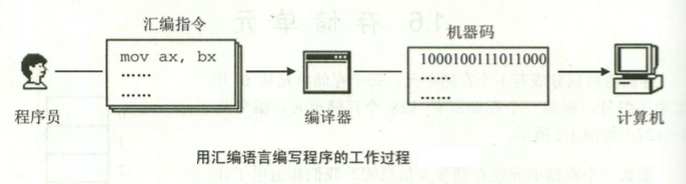
\includegraphics[width=4in]{ch01/fig/asm_process}
\end{figure}
\end{frame}
%
\begin{frame}\ft{存储单元}
存储器被划分为若干个存储单元,每个存储单元从$0$开始顺序编号。例如,假设一个存储器,编号从$0\sim 127$,如下图:
\begin{figure}
\centering
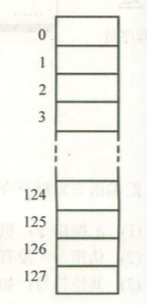
\includegraphics[width=1in]{ch01/fig/cunchudanyuan}
\end{figure}
\end{frame}
%
\begin{frame}\ft{存储单元}

几个概念:

\begin{itemize}
	\item \red{比特(Bit)} \quad 计算机的最小信息单位 \\[.1in]
	\item \red{字节(Byte)} \\[.1in]
	\begin{itemize}
		\item   8个Bit组成1个Byte \\[.1in]
		\item   一个存储单元可存储一个字节,存储器的容量以\red{字节}为最小单位来计算 \\[.1in]
		\item   对于拥有128个存储单元的存储器,其容量为128个字节
	\end{itemize}
	
\end{itemize}
 
对于大容量的存储器,还用以下单位来计算容量(以下用B来代表Byte):
\begin{AutoMultiColItemize}
\item \lstinline|1 KB = 1024 B|   (千)
\item \lstinline|1 MB = 1024 KB|  (兆)
\item \lstinline|1 GB = 1024 KB|  (吉)
\item \lstinline|1 TB = 1024 GB|  (太)
\end{AutoMultiColItemize}
\end{frame}
%
\begin{frame}\ft{CPU对存储器的读写}
\begin{itemize}
\item 首先要指定单元地址。\\[0.1in]
\item 还需要指明\\[0.1in]
\begin{itemize}
	\item 对哪一个存储器进行操作\\[0.1in]
	\item 进行哪种操作\\[0.1in]
	\item 是从中读取数据,还是向里面写入数据
\end{itemize}

\end{itemize}
\end{frame}
%
\begin{frame}\ft{CPU对存储器的读写}
CPU要想进行数据的读写,必须与存储器进行以下3类信息的交互: 

\begin{itemize}
\item \red{地址信息} \quad 存储单元的地址\\[0.1in]
\item \red{控制信息} \quad 器件的选择,以及读或写的命令\\[0.1in]
\item \red{数据信息} \quad 读或写的数据 

\end{itemize}
\end{frame}
%
\begin{frame}\ft{CPU对存储器的读写}
\begin{wenti}
CPU通过什么将地址、数据和控制信息传给存储器芯片呢?
\end{wenti} \pause 
 
计算机传输的信息都是电信号,电信号当然要用导线传送。在计算机中专门有连接CPU和其它芯片的导线,通常称为总线。根据传送信息的不同,总线从逻辑上分为三类: 

\begin{itemize}
\item \red{地址总线} 
\item \red{控制总线}
\item \red{数据总线}
\end{itemize}
\end{frame}
%
\begin{frame}\ft{CPU从内存中读取数据}
\begin{figure}
\centering
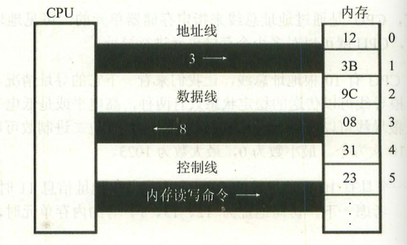
\includegraphics[width=2.5in]{ch01/fig/cpu_read}
\end{figure}
\begin{enumerate}
\item CPU通过\purple{地址总线}将\purple{地址信息$3$}发出;
\item CPU通过\purple{控制总线}发出内存\purple{读命令},选中存储器芯片,并通知它,将要从中读取数据;
\item 存储器将$3$号单元的数据$8$通过\purple{数据总线}送入CPU。
\end{enumerate}
\end{frame}
%
\begin{frame}\ft{CPU对存储器的读写}
写操作与读操作的步骤类似。如向$3$号单元写入数据26。\vspace{0.1in}

\begin{enumerate}
\item CPU通过\purple{地址总线}将\purple{地址信息$3$}发出;
\item CPU通过\purple{控制总线}发出内存\purple{写命令},选中存储器芯片,并通知它,将要从中写入数据;
\item CPU通过\purple{数据总线}将数据$26$送入内存的$3$号单元中。
\end{enumerate}
\end{frame}
%
\begin{frame}\ft{CPU对存储器的读写}
\begin{wenti}
我们知道了CPU如何进行数据的读写。那么,我们又如何命令计算机进行数据的读写呢?
\end{wenti}\pause \vspace{0.1in}

要让计算机工作,应向它输入能驱动其进行工作的电平信息,即机器码。\vspace{0.1in}

\begin{enumerate}
\item[] 机器指令:1010 0001 0000 0011 0000 0000
\item[] 汇编指令:mov ax, [3]
\item[] 含义:传送3号单元的内容入ax。
\end{enumerate}
\end{frame}

\begin{frame}\ft{地址总线}
\begin{itemize}
\item 
CPU通过地址总线指定存储器单元。由此可见,地址总线能传送多少个不同的信息,CPU就可以对多少个存储单元进行寻址。\pause \\[0.1in]
\item 
现假设一个CPU有10根地址总线,可以传送10位二进制数据,共$2^{10}$个不同数据,最小为$0$,最大为$1023$。\pause \\[0.1in]
\item 
一个CPU有$N$根地址线,则称CPU的地址总线的宽度为$N$,最多可以寻找$2^N$个内存单元。
\end{itemize}
\end{frame}
%
\begin{frame}\ft{地址总线}

\begin{figure}
\centering
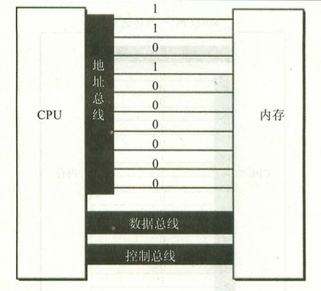
\includegraphics[width=2.5in]{ch01/fig/dizhizongxian}
\caption{地址总线发送的地址信息}
\end{figure}

\end{frame}
%
\begin{frame}\ft{数据总线}
 
CPU与内存和其它器件之间的数据传输通过数据总线来进行。数据总线的宽度决定了CPU与外界的数据传输速度。 
\end{frame}

\begin{frame}\ft{数据总线}

\begin{figure}
\centering
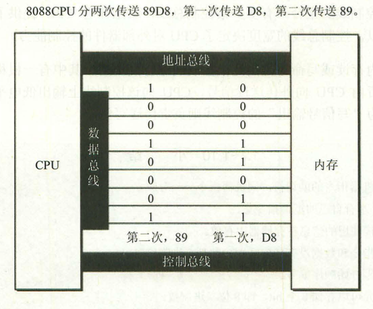
\includegraphics[width=2.5in]{ch01/fig/shujuzongxian1}
\caption{8根数据总线一次可传输一个字节}
\end{figure}

\end{frame}
%
\begin{frame}\ft{数据总线}

\begin{figure}
\centering
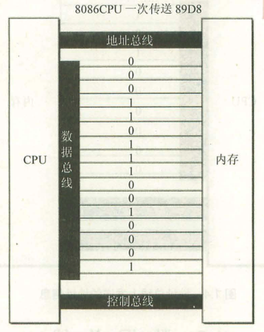
\includegraphics[width=2.in]{ch01/fig/shujuzongxian2}
\caption{16根数据总线一次可传输两个字节}
\end{figure}

\end{frame}

\begin{frame}\ft{控制总线}
 
CPU对外部器件的控制通过控制总线来进行。有多少根控制总线,就意味着CPU提供了对外部器件的多少种控制。因此,控制总线的宽度决定了CPU对外部器件的控制能力。 

\end{frame}

\begin{frame}\ft{寄存器}
一个典型的CPU由运算器、控制器、寄存器等器件构成,这些器件通过内部总线相连。 内部总线实现CPU内部各个器件之间的联系,而外部总线实现CPU与主板上其它器件的联系。 

在CPU中:
\begin{itemize}
\item 运算器进行信息处理;
\item 寄存器进行信息存储;
\item 控制器控制各种器件进行工作;
\item 内部总线连接各种器件,在它们之间进行数据的传送。
\end{itemize}
\end{frame}
%
\begin{frame}\ft{寄存器}
寄存器是CPU中程序员可以用指令读写的部件,程序员通过改变各种寄存器中的内容来实现对CPU的控制。\vspace{0.1in}

不同的CPU,寄存器的个数、结构不尽相同。8086CPU有14个寄存器,每个寄存器都有一个名称,分别是
$$
\mbox{AX、BX、CX、DX、SI、DI、SP、BP、IP、CS、SS、DS、ES、PSW。}
$$
\end{frame}

\begin{frame}\ft{通用寄存器}
8086CPU的所有寄存器都是16位的,可以存放两个字节。\vspace{0.1in}

AX、BX、CX、DX这四个寄存器通常用来存放一般性的数据,被称为通用寄存器。

\begin{figure}
\centering
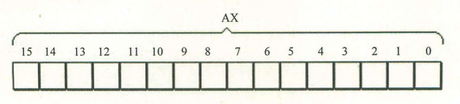
\includegraphics[width=3.5in]{ch01/fig/tongyongjicunqi1}
\caption{16位寄存器的逻辑结构}
\end{figure}


\end{frame}

\begin{frame}\ft{通用寄存器}
\begin{figure}
\centering
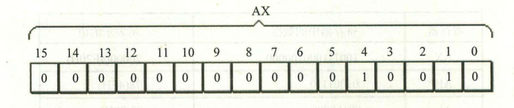
\includegraphics[width=3.5in]{ch01/fig/tongyongjicunqi2}
\caption{$(10010)_2$在寄存器AX中的存储}
\end{figure}
 
\begin{figure}
\centering
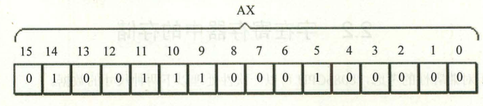
\includegraphics[width=3.5in]{ch01/fig/tongyongjicunqi3}
\caption{$(100111000100000)_2$在寄存器AX中的存储}
\end{figure}
\end{frame}
%
%
%
\begin{frame}\ft{通用寄存器}
\begin{figure}
\centering
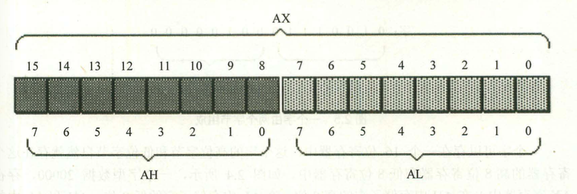
\includegraphics[width=3.5in]{ch01/fig/tongyongjicunqi4}
\caption{16位寄存器可分为两个8位寄存器}
\end{figure}
\end{frame}

\begin{frame}\ft{几条汇编指令}
\begin{figure}
\centering
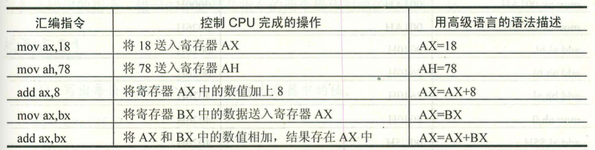
\includegraphics[width=4.5in]{ch01/fig/huibianzhiling1}
\caption{汇编指令举例}
\end{figure}
\end{frame}

\begin{frame}\ft{物理地址}
CPU访问内存单元时,要给出内存单元的地址。所有的内存单元构成的存储空间是一个一维的线性空间,每一个内存单元在这个空间中都有唯一的地址,称为物理地址。\vspace{0.1in}

CPU通过地址总线送入存储器的,必须是一个内存单元的物理地址。在CPU向地址总线上发出物理地址之前,必须要在内部先形成这个物理地址。不同的CPU可以有不同的形成物理地址的方式。
\end{frame}

%\begin{frame}\ft{16位结构的CPU}
%16位结构描述了一个CPU具有以下几个方面的结构特性。\vspace{0.1in}
%
%\begin{itemize}
%\item 运算器一次最多可以处理16位的数据;\\[0.1in]
%\item 寄存器的最大宽度为16位;\\[0.1in]
%\item 寄存器与运算器之间的通路是16位。
%\end{itemize}
%\end{frame}
%
%\begin{frame}\ft{8086CPU给出物理地址的方法}
%8086CPU有20位地址总线,可以传送20位地址,达到1MB寻址能力。\vspace{0.1in}
%
%同时8086CPU是16位结构,在内部一次处理、传输、暂存的地址是16位。
%\vspace{0.1in}
%
%从8086CPU的内部结构来看,若将地址从内部简单出发,只能送出16位的地址,表现出的寻址能力只有64KB。\pause 
%\vspace{0.1in}
%
%\red{8086CPU采用一种在内部用两个16位地址合成的方法来形成一个20位的物理地址。}
%\end{frame}
%
%\begin{frame}\ft{8086CPU给出物理地址的方法}
%\begin{figure}
%\centering
%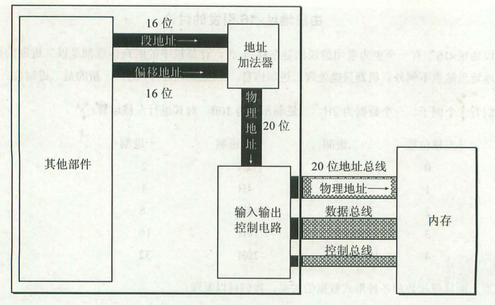
\includegraphics[width=4in]{ch01/fig/xunzhi}
%\caption{8086CPU相关部件的逻辑结构}
%\end{figure}
%\end{frame}
%
%\begin{frame}\ft{8086CPU给出物理地址的方法}
%\begin{figure}
%\centering
%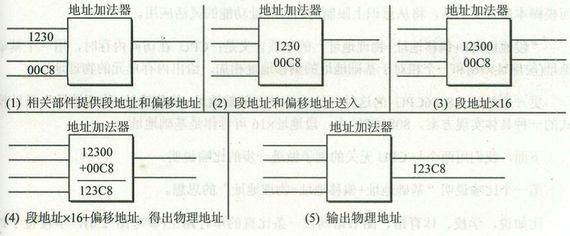
\includegraphics[width=4in]{ch01/fig/xunzhi1}
%\caption{地址加法器的工作过程(物理地址=段地址$\times$16+偏移地址)}
%\end{figure}
%
%\end{frame}
%%
%\begin{frame}\ft{段的概念}
%\begin{figure}
%\centering
%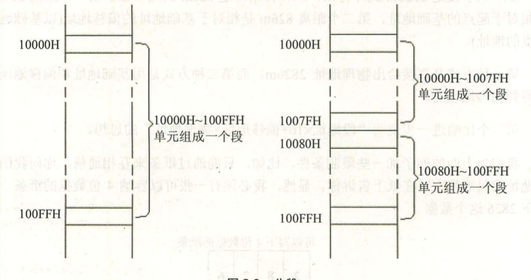
\includegraphics[width=4in]{ch01/fig/duan}
%\caption{内存并没有分段,段的划分来自于CPU,由于8086CPU用“基础地址(段地址$\times$16)+偏移地址”的方式给出内存单元的物理地址,使得我们可以用分段的方式来管理内存。}
%\end{figure}
%\end{frame}
%
%\begin{frame}\ft{段寄存器}
%8086CPU在访问内存时由相关部件提供内存单元的段地址和偏移地址,送入地址加法器合成物理地址。\vspace{0.1in}
%
%段地址在8086CPU的段寄存器中存放。8086CPU有4个段寄存器:CS、DS、SS、ES。\vspace{0.1in}
%
%8086CPU访问内存时由这四个段寄存器提供内存单元的段地址。
%\end{frame}
%
%\begin{frame}\ft{CS和IP}
%CS和IP是8086CPU中两个最关键的寄存器,指示CPU当前要读取指令的地址。
%\vspace{0.1in}
%
%CS为代码段寄存器,IP为指令指针寄存器。
%\vspace{0.1in}
%
%设CS的内容为$M$,IP的内容为$N$,则8086CPU将从内存$M\times16+N$单元开始,读取一条指令并执行。\pause \vspace{0.2in}
%
%\red{以下展示8086CPU读取、执行命令的工作原理:}
%\end{frame}
%
%\begin{frame}\ft{CS和IP}
%
%\begin{figure}
%\centering
%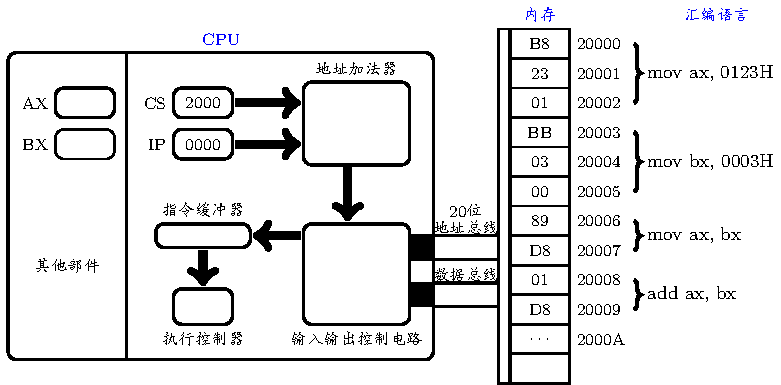
\includegraphics[width=4.5in]{Tikz/csip1}
%\caption{初始状态:CPU将从内存2000:0000处读取指令}
%\end{figure}
%
%\end{frame}
%
%\begin{frame}\ft{CS和IP}
%\begin{figure}
%\centering
%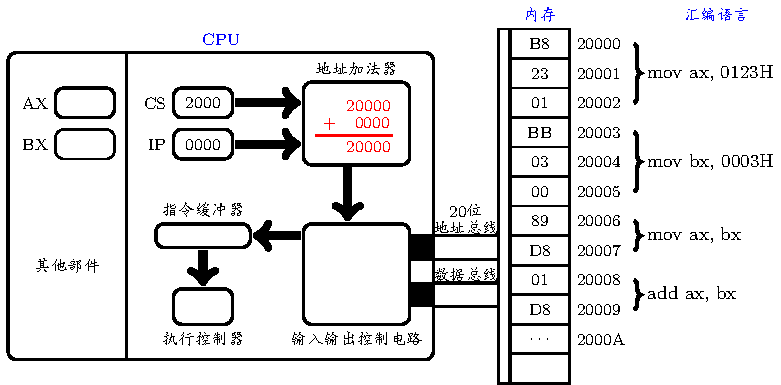
\includegraphics[width=4.5in]{Tikz/csip2}
%\caption{CS、IP中的内容送入地址加法器,形成物理地址}
%\end{figure}
%
%\end{frame}
%
%
%\begin{frame}\ft{CS和IP}
%\begin{figure}
%\centering
%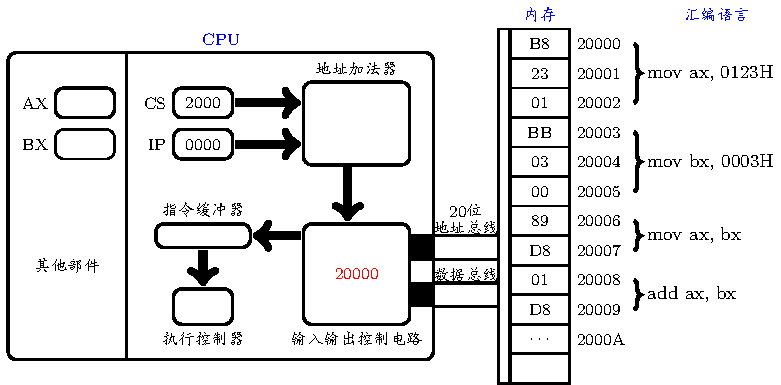
\includegraphics[width=4.5in]{Tikz/csip3}
%\caption{地址加法器将物理地址送至输入输出控制电路}
%\end{figure}
%
%\end{frame}
%
%\begin{frame}\ft{CS和IP}
%\begin{figure}
%\centering
%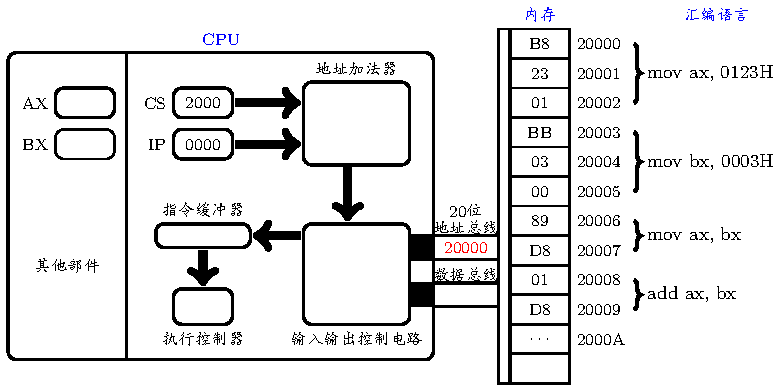
\includegraphics[width=4.5in]{Tikz/csip4}
%\caption{输入输出控制电路将物理地址送上地址总线}
%\end{figure}
%
%\end{frame}
%
%\begin{frame}\ft{CS和IP}
%\begin{figure}
%\centering
%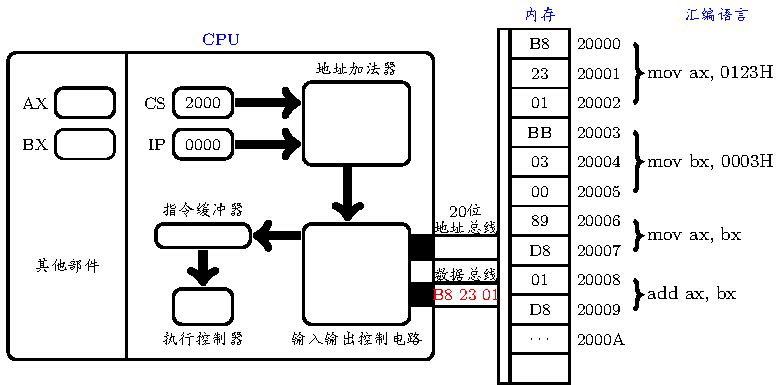
\includegraphics[width=4.5in]{Tikz/csip5}
%\caption{将内存20000H单元开始存放的机器指令B8~23~01通过数据总线送入CPU}
%\end{figure}
%
%\end{frame}
%
%
%\begin{frame}\ft{CS和IP}
%\begin{figure}
%\centering
%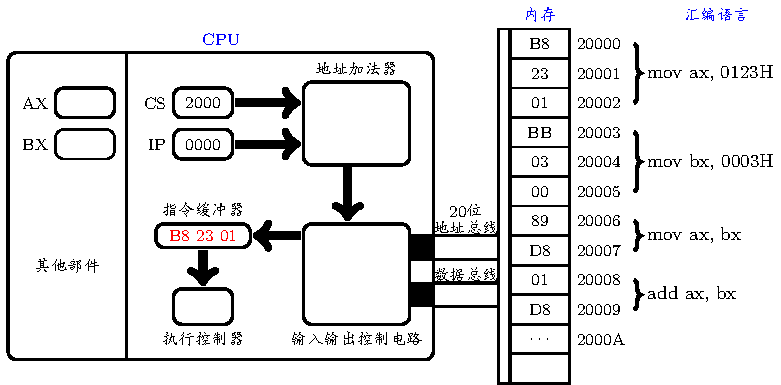
\includegraphics[width=4.5in]{Tikz/csip6}
%\caption{输入输出控制电路将机器指令B8~23~01送入指令缓冲器}
%\end{figure}
%
%\end{frame}
%
%\begin{frame}\ft{CS和IP}
%\begin{figure}
%\centering
%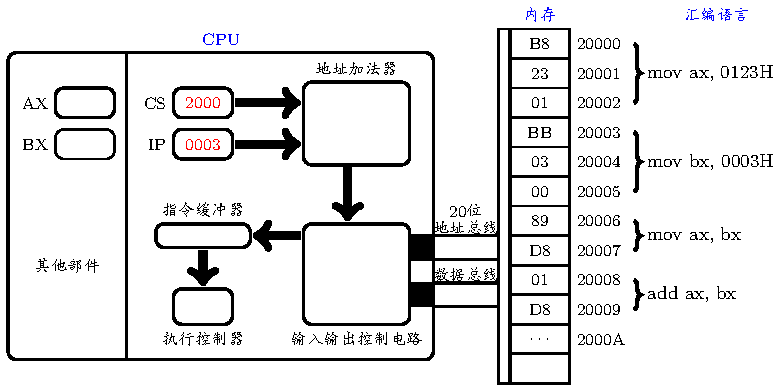
\includegraphics[width=4.5in]{Tikz/csip7}
%\caption{IP中的值自动增加:读取一条指令后,IP中的值自动增加,以使CPU可以读取下一条指令。因当前读入的指令B8~23~01为3个字节,故IP中的值加3。}
%\end{figure}
%
%\end{frame}
%
%
%\begin{frame}\ft{CS和IP}
%\begin{figure}
%\centering
%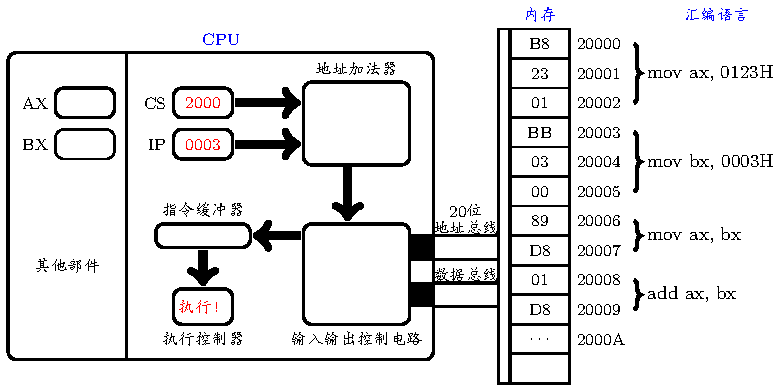
\includegraphics[width=4.5in]{Tikz/csip8}
%\caption{执行控制器执行指令B8~23~01,即mov ax, 0123H}
%\end{figure}
%
%\end{frame}
%
%\begin{frame}\ft{CS和IP}
%\begin{figure}
%\centering
%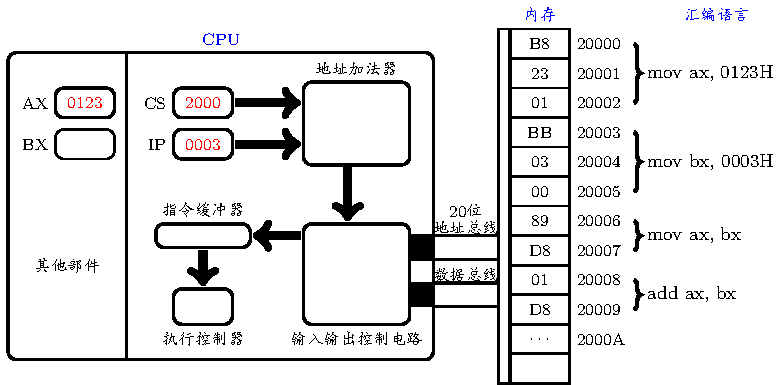
\includegraphics[width=4.5in]{Tikz/csip9}
%\caption{指令B8~23~01被执行后AX中的内容为0123H,此时CPU将从内存单元2000:0003处读取指令。}
%\end{figure}
%
%\end{frame}
%
%\begin{frame}\ft{CS和IP}
%\begin{figure}
%\centering
%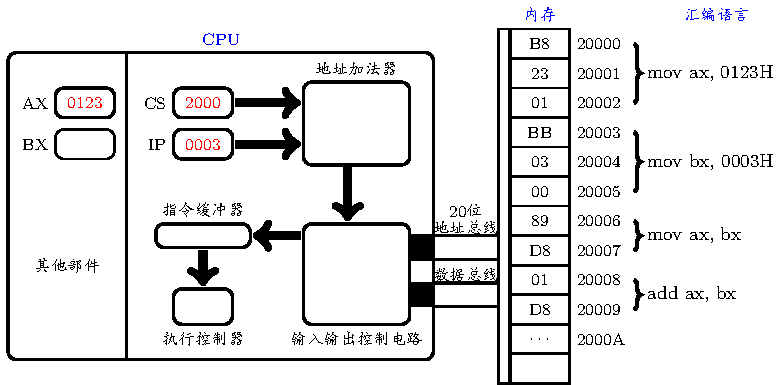
\includegraphics[width=4.5in]{Tikz/csip9}
%\caption{CS:2000H,IP:0003H,CPU将读取指令BB~03~00}
%\end{figure}
%
%\end{frame}
%
%\begin{frame}\ft{CS和IP}
%\begin{figure}
%\centering
%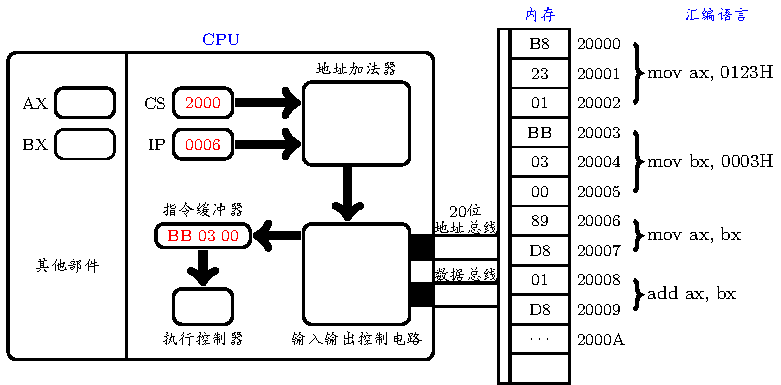
\includegraphics[width=4.5in]{Tikz/csip10}
%\caption{CPU读取指令BB~03~00入指令缓冲器,IP中的值加3。}
%\end{figure}
%
%\end{frame}
%
%
%
%
%\begin{frame}\ft{CS和IP}
%\begin{figure}
%\centering
%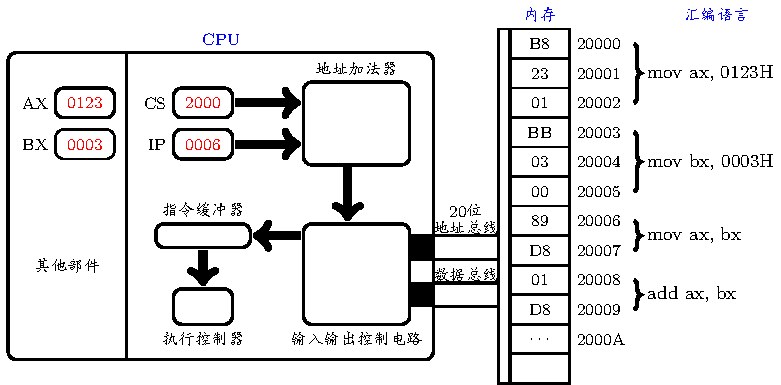
\includegraphics[width=4.5in]{Tikz/csip11}
%\caption{执行指令BB~03~00,即mov bx, 0003H}
%\end{figure}
%
%\end{frame}
%
%
%\begin{frame}\ft{CS和IP}
%\begin{figure}
%\centering
%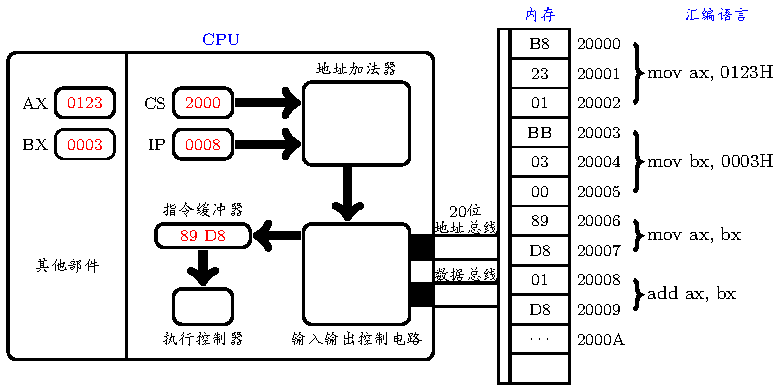
\includegraphics[width=4.5in]{Tikz/csip12}
%\caption{CPU从内存20006H处读取指令89~D8如指令缓冲器,IP中的值加2。}
%\end{figure}
%
%\end{frame}
%
%\begin{frame}\ft{CS和IP}
%\begin{figure}
%\centering
%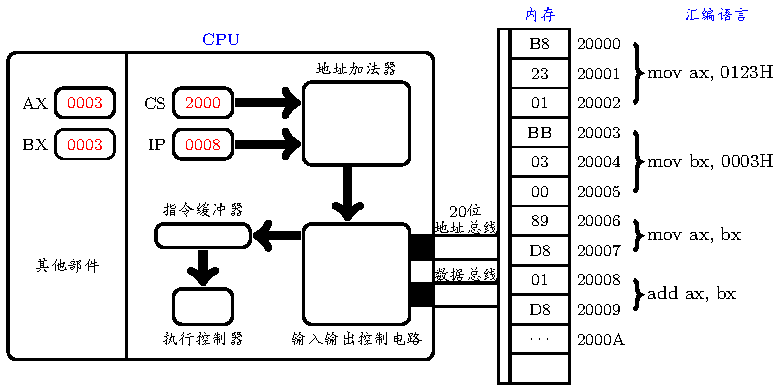
\includegraphics[width=4.5in]{Tikz/csip13}
%\caption{执行指令89~D8,即mov ax, bx后,AX中的内容为0003H}
%\end{figure}
%
%\end{frame}
%
%\begin{frame}\ft{CS和IP}
%\begin{figure}
%\centering
%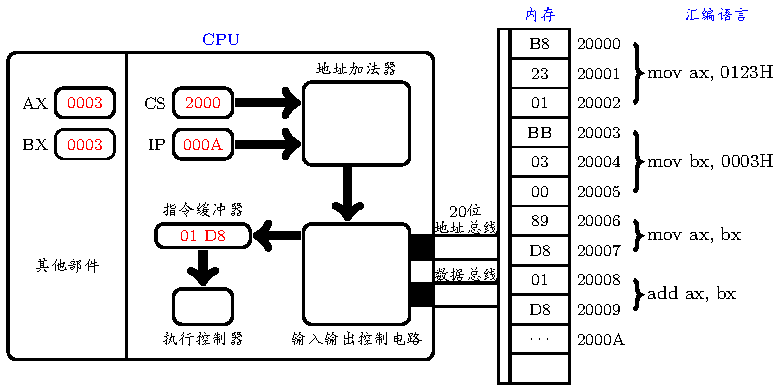
\includegraphics[width=4.5in]{Tikz/csip14}
%\caption{CPU从内存20008H处读取指令01~D8如指令缓冲器,IP中的值加2。}
%\end{figure}
%
%\end{frame}
%
%\begin{frame}\ft{CS和IP}
%\begin{figure}
%\centering
%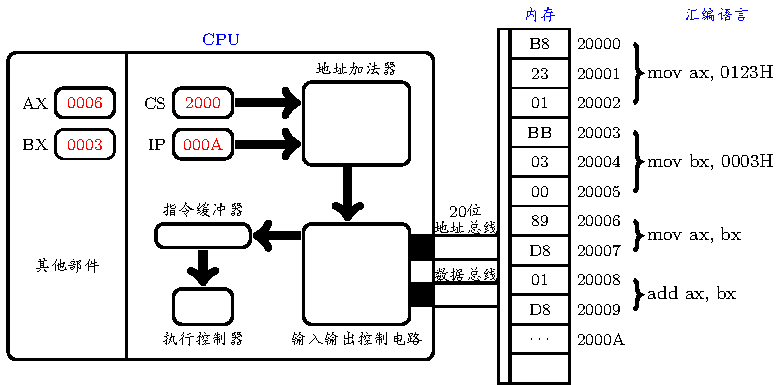
\includegraphics[width=4.5in]{Tikz/csip15}
%\caption{执行指令01~D8,即add ax, bx后,AX中的内容为0006H}
%\end{figure}
%\end{frame}
%
%\begin{frame}\ft{CS和IP}
%8086CPU的工作过程:\vspace{0.1in}
%
%\begin{itemize}
%\item[(1)] 从CS:IP指向的内存单元读取指令,读取的指令进入指令缓冲器;\\[0.1in]
%\item[(2)] IP=IP+所读取指令的长度,从而指向下一条指令;\\[0.1in]
%\item[(3)] 执行指令。转至步骤(1),重复整个过程。
%\end{itemize}
%\end{frame}
%
%\begin{frame}\ft{CS和IP}
%CPU刚开始工作时,CS和IP被设置为CS=FFFFH,IP=0000H,即开机时,CPU从内存FFFF0H单元中读取指令执行,FFFF0H单元中的指令是开机后执行的第一条指令。
%\end{frame}
%
%
%
